\section{Post-Training}

\begin{figure}[H]
\centering
\resizebox{1.0\textwidth}{!}{%
\begin{tikzpicture}[
    stage/.style={
        draw=black,
        line width=0.5pt,
        fill=white,
        rounded corners=4pt,
        minimum width=2.55cm,
        minimum height=0.95cm,
        align=center,
        font=\small
    },
    milestone/.style={
        stage,
        line width=1.4pt,
        font=\small\bfseries
    },
    flowarrow/.style={-{Latex[length=2.0mm]}, line width=0.45pt}
]
\path[fill=gray!12, rounded corners=10pt]
    (-2.10,-2.90) rectangle (14.35,1.10);

\node[stage] (pre-train) at (0,0) {Pre-Training};
\node[stage] (anneal) at (3.05,0) {High-Quality\\Annealing};
\node[milestone] (base) at (6.10,0) {Loopie\\Base};
\node[stage] (spt) at (6.10,-1.70) {Supervised\\Pre-Training};
\node[stage] (mathrl) at (9.15,-1.70) {Math RL};
\node[milestone] (thinking) at (12.20,-1.70) {Loopie\\Thinking};

\draw[flowarrow] (pre-train.east) -- (anneal.west);
\draw[flowarrow] (anneal.east) -- (base.west);
\draw[flowarrow] (base.south) -- (spt.north);
\draw[flowarrow] (spt.east) -- (mathrl.west);
\draw[flowarrow] (mathrl.east) -- (thinking.west);
\end{tikzpicture}%
}
\caption{Overview of the Loopie training pipeline. The model is first pre-trained and annealed to produce \textbf{Loopie Base}, which then undergoes supervised pre-training and Math RL to produce \textbf{Loopie Thinking}.}
\label{fig:posttraining-pipeline}
\end{figure}

Loopie's post-training recipe consists of two main stages following Stage 2 high-quality annealing. First, we introduce a supervised pre-training stage in which we continue training the model on 2T tokens of instruction-following, reasoning, coding, mathematics, and tool-use data, allowing the base model to acquire broad task-following and problem-solving capabilities while preserving the knowledge and general capabilities learned during pre-training. Second, we apply large-scale reinforcement learning to further enhance Loopie's reasoning capabilities, improve its long-horizon problem solving, and align the model so that it produces reliable thinking traces. Together, these stages transform \textbf{Loopie Base} into the final \textbf{Loopie Thinking} model.

\subsection{Supervised Pre-Training}
\label{sec:spt}

We introduce \emph{supervised pre-training} (SPT), a training
regime that combines the supervision pattern of supervised fine-tuning
(SFT) with the optimization scale of language-model pre-training (PT).
SPT uses exactly the same training data and token-level objective as
SFT: prompt and context tokens are excluded from the loss, and only
supervised target tokens contribute to optimization. Unlike conventional
SFT, however, SPT uses global batch sizes, sequence lengths, and token
budgets typical of language-model pre-training.

\begin{table}[H]
\centering
\caption{
Comparison of supervised pre-training (SPT), conventional supervised
fine-tuning (SFT), and pre-training (PT). The SPT column reports the
representative configuration used for \textsc{Loopie}.
$\uparrow$, $\downarrow$, and $\approx$ indicate improvement,
degradation, and no material change, respectively, relative to the
corresponding starting checkpoint. Stability entries summarize our
observations over the evaluated training horizon rather than universal
guarantees.
}
\label{tab:spt-comparison}
\small
\setlength{\tabcolsep}{5pt}
\renewcommand{\arraystretch}{1.16}
\begin{tabularx}{
    \textwidth
}{
    @{}
    >{\raggedright\arraybackslash}p{0.29\textwidth}
    >{\centering\arraybackslash}X
    >{\centering\arraybackslash}X
    >{\centering\arraybackslash}X
    @{}
}
\toprule
&
\textbf{SPT}
&
\textbf{SFT}
&
\textbf{PT}
\\
\midrule

Loss function
&
Cross-entropy
&
Cross-entropy
&
Cross-entropy
\\

Loss-bearing positions
&
Supervised target tokens only
&
Supervised target tokens only
&
All non-padding tokens
\\

Pre-training metrics
&
$\uparrow$
&
$\downarrow$
&
$\uparrow$
\\

Reasoning metrics
&
$\uparrow$
&
$\uparrow$
&
$\approx$
\\

Overfitting after multiple epochs
&
Not observed
&
Observed
&
Not observed
\\

Global batch size
&
$\geq 1{,}024$
&
$32$--$128$
&
$\geq 1{,}024$
\\

Sequence length
&
$\geq 128\,\mathrm{K}$
&
$8$--$32\,\mathrm{K}$
&
$4$--$8\,\mathrm{K}$
\\

Nominal token positions per batch
&
$\geq 128\,\mathrm{M}$
&
$128\,\mathrm{K}$--$1\,\mathrm{M}$
&
$8$--$32\,\mathrm{M}$
\\

Total training token budget
&
$\geq 2\,\mathrm{T}$
&
$10$--$100\,\mathrm{B}$
&
$\geq 4\,\mathrm{T}$
\\

\bottomrule
\end{tabularx}

\vspace{2pt}
\end{table}


SPT separates two design choices that are commonly coupled:
(i) which tokens contribute to the training loss, and
(ii) the scale at which optimization is performed.
SFT and SPT share the former choice, whereas PT and SPT share the
latter. Consequently, SPT does not interpolate between an SFT loss and
a PT loss. Instead, it applies an SFT-style supervised objective in a
PT-scale optimization regime.

\paragraph{Training objective.}
Consider a supervised example
$z_i = [c_i; y_i]$, where $c_i$ denotes the input context and $y_i$
denotes the supervised target response. Let $w_{i,t} \in \{0,1\}$ be a
binary loss mask for the token at position $t$. All three training
regimes use token-level cross-entropy:
%
\begin{equation*}
\mathcal{L}_{\mathrm{CE}}(\theta; w)
=
-
\frac{
    \displaystyle
    \sum_{i=1}^{B}
    \sum_{t=1}^{T_i}
    w_{i,t}
    \log p_{\theta}
    \left(
        z_{i,t} \mid z_{i,<t}
    \right)
}{
    \displaystyle
    \sum_{i=1}^{B}
    \sum_{t=1}^{T_i}
    w_{i,t}
}.
\label{eq:spt-loss}
\end{equation*}
%
For both SPT and SFT, $w_{i,t}=1$ only when $z_{i,t}$ belongs to the
supervised target $y_i$; prompt, context, and padding positions are
masked out. In conventional PT, by contrast, $w_{i,t}=1$ for every non-padding token. Thus, all three regimes employ the same cross-entropy loss, but differ in the positions to which the loss is applied and in the scale of optimization.

Table~\ref{tab:spt-comparison} summarizes these distinctions. For representative SFT settings, including global batch sizes, training token counts, and sequence lengths, we primarily follow the configurations reported for OLMo 3, the Nemotron 3 series, and Step-3.5-Flash~\citep{olmo2026olmo3,nvidia2025nemotron3nanoopen,bercovich2025llamanemotronefficientreasoningmodels,nvidia2026nemotron3superopen,nvidia2026nemotron3ultraopen,huang2026step35flashopen}. We use
\emph{pre-training metrics} to refer to metrics that evaluate general base-model capabilities and \emph{reasoning metrics} to refer to metrics that primarily evaluate performance on challenging reasoning tasks, such as competition-level mathematics and coding problems. In our experiments, SPT improves performance on both types of metrics simultaneously. In contrast, the conventional SFT baseline only improves performance on reasoning metrics but degrades performance on pre-training metrics, whereas PT improves pre-training metrics performance while leaving performance on reasoning metrics approximately unchanged.

\begin{figure}[!t]
\centering
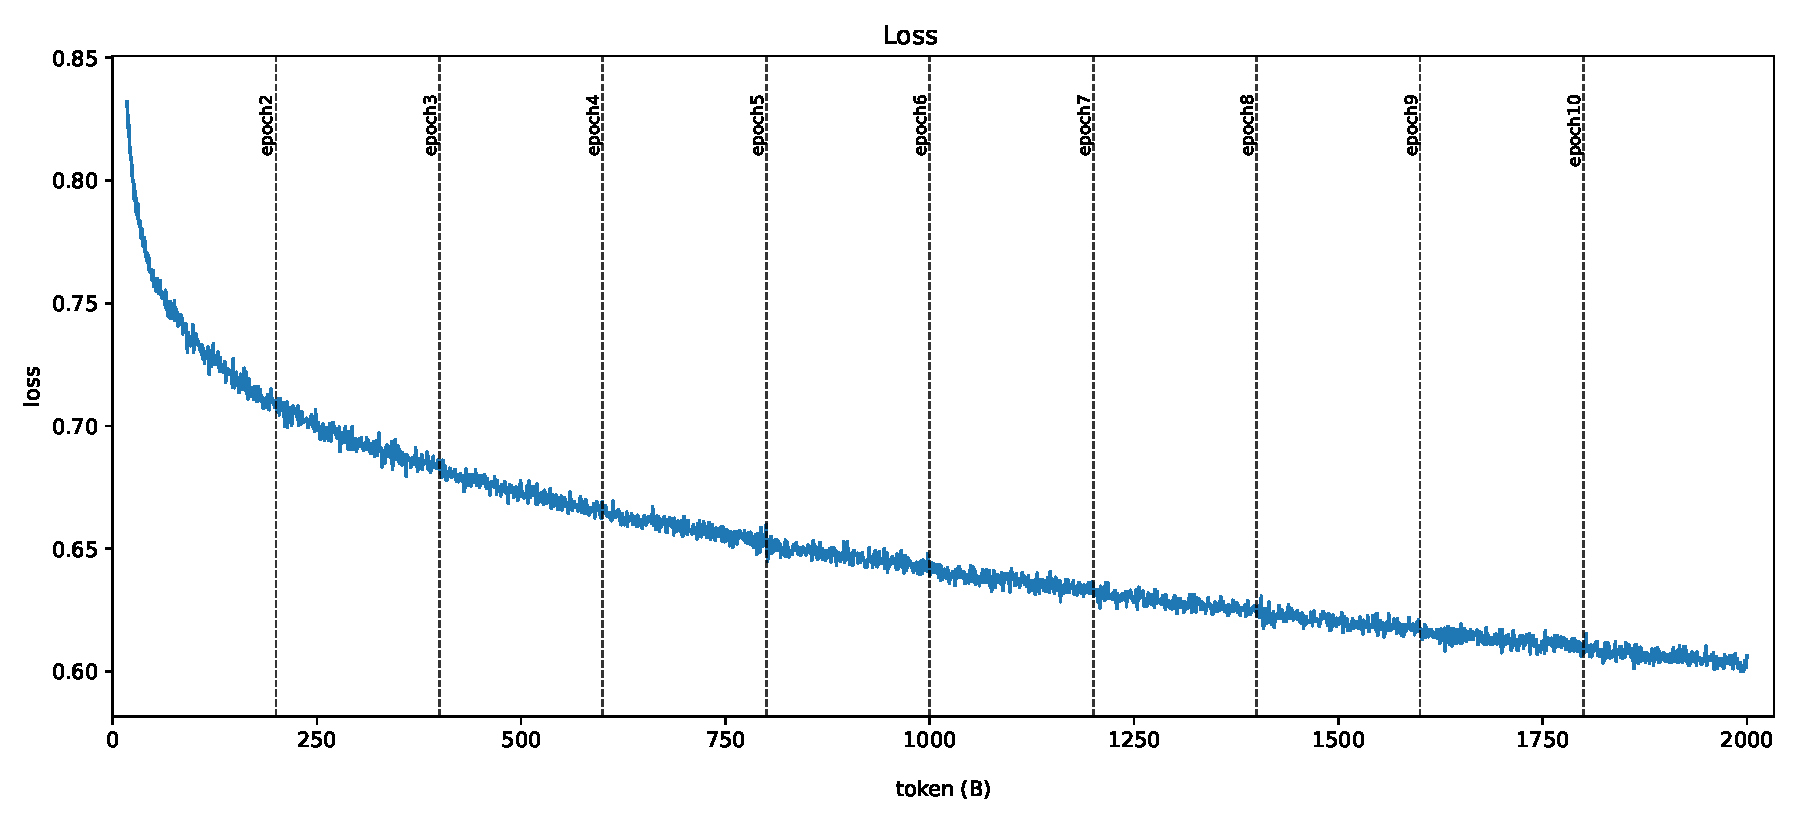
\includegraphics[width=0.8\textwidth]{figures/loss.pdf}
\caption{Training loss for Loopie-6B-A0.6B during supervised pre-training. Because the evaluation and training loss curves nearly overlap, only the training loss curve is shown. Over 10 epochs of supervised pre-training on a total of 2 trillion tokens, the loss decreases smoothly, with no loss cliff observed at epoch boundaries.}
\end{figure}


\begin{figure}[H]
\centering
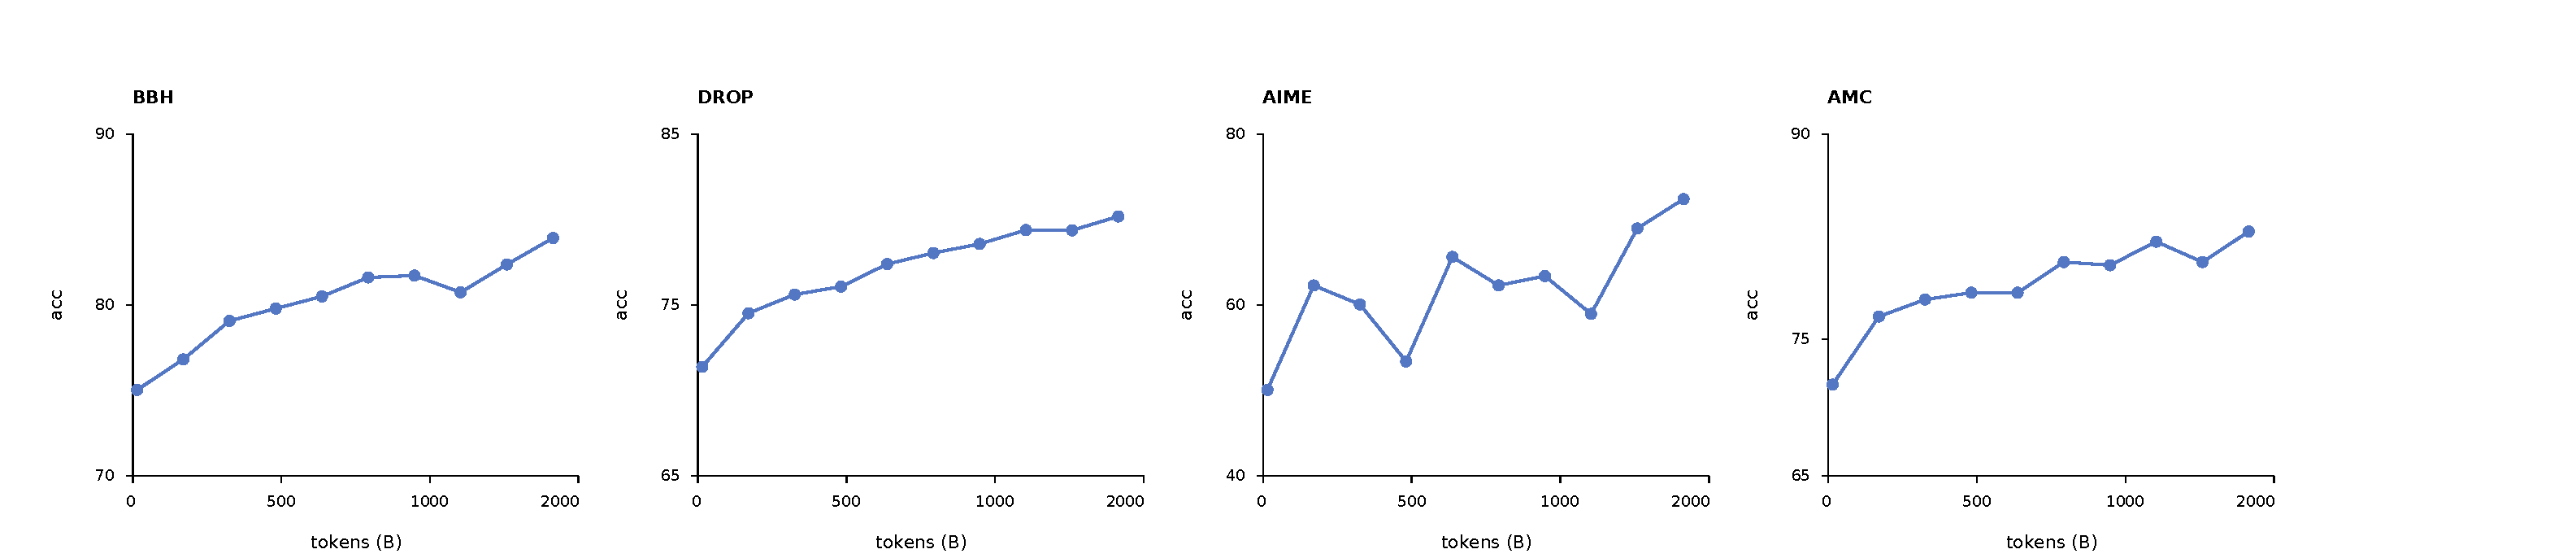
\includegraphics[width=1.08\textwidth]{figures/spt_ds.pdf}
\caption{Trends in reasoning metrics during supervised pre-training. Throughout training on 2 trillion tokens, performance on the reasoning metrics continues to improve, with no sign of slowing.}
\label{fig:spt-reasoning}
\end{figure}







\paragraph{Pre-training-scale optimization over supervised data.}
SPT processes 128 million tokens per global batch, approximately 1,000 times the number processed per batch in conventional SFT. This makes overfitting much less likely in SPT than in standard SFT. This scale gives SPT distinct training dynamics, consistent with observations that optimization hyperparameters and scaling behavior can change in large-language-model training regimes~\citep{jin2023rethinkinglearningratetuning}. Under SPT, the model can be trained smoothly for substantially more epochs without showing signs of overfitting, such as abrupt drops in loss at epoch boundaries. At the same time, performance on downstream metrics continues to improve steadily. In addition, SPT mitigates catastrophic forgetting~\citep{wu2024mitigating}, which is a major drawback of conventional SFT and typically causes substantial degradation of the general knowledge acquired during pre-training. Notably, SPT not only avoids this degradation but also further improves general-knowledge performance.

As shown in Figure~\ref{fig:spt-pt}, SPT consistently improves performance on downstream pre-training metrics, including ARC-Challenge and MMLU, throughout approximately 10 epochs of training on 2T tokens. This finding challenges the conventional view that SFT leads to catastrophic forgetting.

\begin{figure}[H]
\centering
\hspace*{-4mm}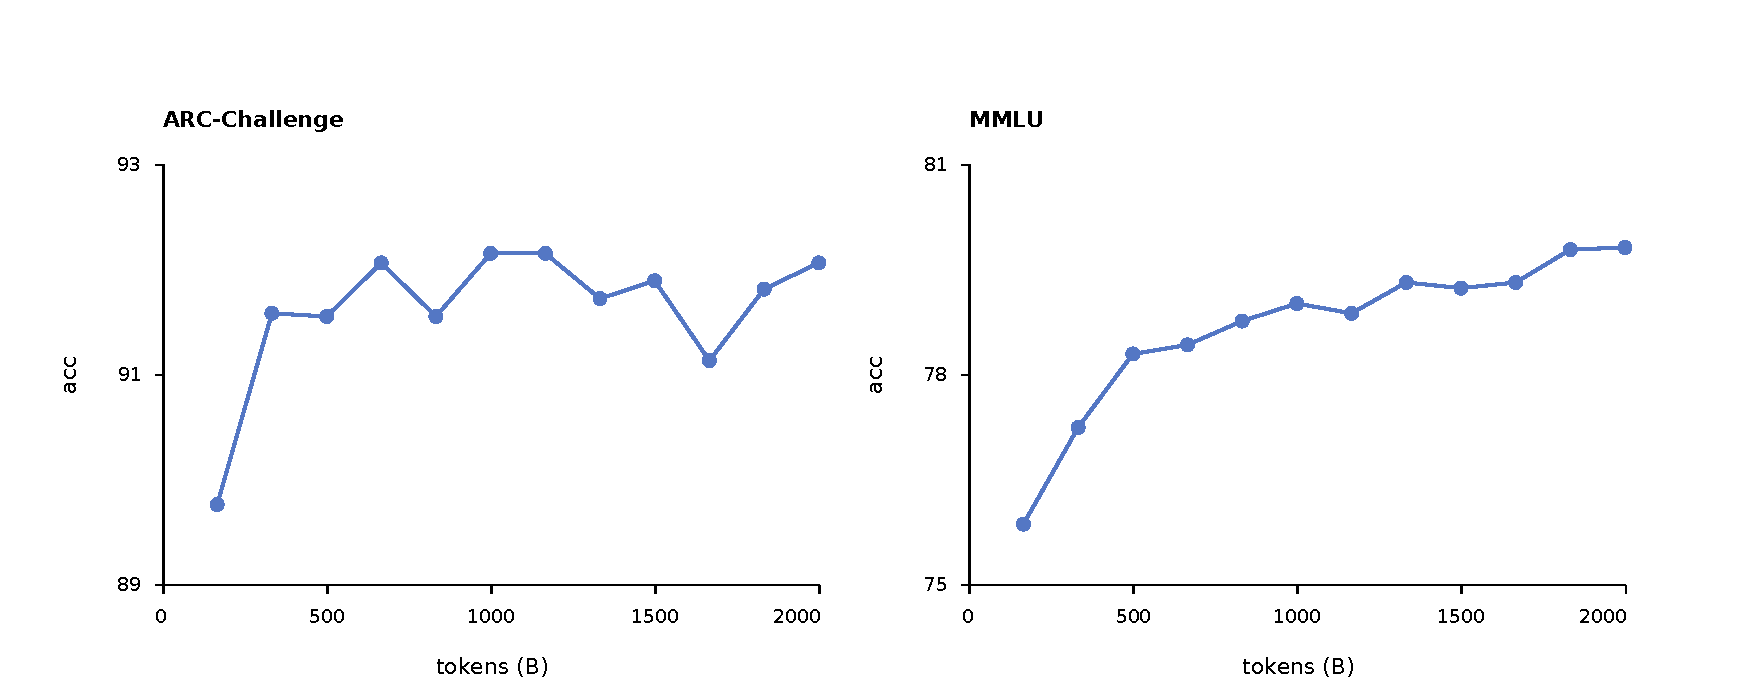
\includegraphics[width=0.85\textwidth]{figures/spt.pdf}\hspace*{4mm}
\caption{Trends in pre-training metrics during supervised pre-training. ARC-Challenge represents general reasoning performance, while MMLU represents general knowledge performance. Throughout training on 2 trillion tokens, performance on the pre-training metrics does not degrade; instead, it continues to improve.}
\label{fig:spt-pt}
\end{figure}

Simply running a conventional SFT configuration for more epochs does not reproduce the optimization regime of SPT. Conventional-scale SFT often begins to overfit between the second and fourth epochs. In small-batch SFT, each epoch involves many parameter updates computed from small batches, and repeated exposure to the same examples can lead to rapid specialization and memorization. In contrast, every SPT update aggregates supervision from more than one thousand sequences and over one hundred million nominal token positions. We hypothesize that this broad gradient aggregation, together with long contexts and a large token budget, mitigates the overly narrow specialization commonly observed during repeated SFT.

\subsection{Reinforcement Learning}
\label{sec:rl}

After SPT, we apply a reinforcement-learning stage to obtain \textbf{Loopie Thinking}. Following prior work, we do not mix data from multiple domains during training because domain-specific length biases may interfere with one another~\citep{chen2026acereasonnemotron,liu2026acereasonnemotron}. We first conduct reinforcement learning on mathematical tasks; once performance saturates, we continue with reinforcement learning on coding tasks.


\paragraph{Algorithm.}
Our optimizer builds on Group Sequence Policy Optimization (GSPO) \citep{zheng2025groupsequencepolicyoptimization}, with the asymmetric clipping and dynamic sampling techniques introduced by DAPO \citep{yu2025dapo}. For each prompt $q$, we sample a group of $G$ completions $\{o_i\}_{i=1}^{G}$ from the old policy $\pi_{\theta_{\mathrm{old}}}$ and score each completion using a verifier, yielding outcome rewards $\{R_i\}_{i=1}^{G}$.
We estimate sequence-level advantages by normalizing rewards within the
sampled group:
%
\begin{equation*}
\hat{A}_i
=
\frac{
    R_i - \operatorname{mean}(\{R_j\}_{j=1}^{G})
}{
    \operatorname{std}(\{R_j\}_{j=1}^{G}) + \epsilon
},
\label{eq:rl-group-advantage}
\end{equation*}
%
where $\epsilon$ is a small numerical constant.

Unlike token-level policy optimization, GSPO defines a length-normalized
sequence-level importance ratio:
%
\begin{equation*}
s_i(\theta)
=
\left(
    \frac{\pi_{\theta}(o_i \mid q)}{\pi_{\theta_{\mathrm{old}}}(o_i \mid q)}
\right)^{\frac{1}{|o_i|}}
=
\exp
\left(
    \frac{1}{|o_i|}
    \sum_{t=1}^{|o_i|}
    \log
    \frac{\pi_{\theta}(o_{i,t} \mid q, o_{i,<t})}{\pi_{\theta_{\mathrm{old}}}(o_{i,t} \mid q, o_{i,<t})}
\right).
\end{equation*}
%
That is, $s_i(\theta)$ is the geometric mean of the token-level
importance ratios over the response. The length normalization reduces
the variance of the sequence-level ratio and keeps responses of different
lengths within a comparable numerical range.

The policy is optimized using a sequence-level clipped objective:
%
\begin{equation*}
\mathcal{J}_{\mathrm{RL}}^{\mathrm{GSPO}}(\theta)
=
\mathbb{E}_{
    q \sim \mathcal{D},\,
    \{o_i\}_{i=1}^{G}
    \sim \pi_{\theta_{\mathrm{old}}}(\cdot \mid q)
}
\left[
    \frac{1}{G}
    \sum_{i=1}^{G}
    \min
    \left(
        s_i(\theta)\hat{A}_i,\,
        \operatorname{clip}
        \left(
            s_i(\theta),
            1-\epsilon_{\mathrm{low}},
            1+\epsilon_{\mathrm{high}}
        \right)
        \hat{A}_i
    \right)
\right].
\label{eq:gspo-objective}
\end{equation*}
%
In contrast to token-level clipping, GSPO applies the clipping operation
to the entire response. Consequently, all tokens in the same response
share the same sequence-level importance weight, aligning the unit of
off-policy correction and optimization with the unit of reward.

Following the Clip-Higher strategy, we use
$\epsilon_{\mathrm{high}} > \epsilon_{\mathrm{low}}$.
Under GSPO, this asymmetric clipping is applied to the sequence-level importance ratio rather than individual token-level ratios. The larger upper clipping range allows positively advantaged exploratory responses
to receive stronger probability-increasing updates, while the more
conservative lower clipping range limits excessive probability decreases
for negatively advantaged responses.

We further apply prompt-level dynamic filtering. A prompt is retained only
when its sampled group contains both successful and unsuccessful completions:
%
\begin{equation*}
0
<
\sum_{i=1}^{G}
\mathbf{1}\{R_i = R_{\mathrm{pass}}\}
<
G.
\label{eq:dynamic-filtering}
\end{equation*}
%
Groups that are entirely correct or entirely incorrect provide no useful
relative preference signal for GRPO. We therefore oversample candidate
prompts and filter out such groups until the effective batch is full. This
keeps the optimization focused on prompts that yield non-degenerate policy
gradients.

\paragraph{Training data.}
We use the mathematics and code subsets of the Guru-RL corpus
\citep{cheng2025guru}. The mathematics pool is drawn from the OR1, DAPO, and
DeepScaleR sources \citep{he2025skywork,yu2025dapo,tan2025deepscaler}. The
code pool combines LeetCodeDataset, TACO-Verified, PrimeIntellect/SYNTHETIC-1,
and historical LiveCodeBench training problems
\citep{xia2025leetcodedataset,li2023taco,li2024tacoverified,
mattern2025synthetic1,jain2024livecodebench}. We apply an additional
curation pass that removes malformed prompts, unverifiable answers, flaky
tests, duplicate examples, and examples that substantially overlap with
held-out evaluation sets. Rewards for mathematical problems are computed using
rule-based answer equivalence, whereas rewards for coding problems are computed
using sandboxed unit-test execution.

\paragraph{Training schedule.}
We train in two context-length stages. The first stage uses a maximum response
length of $32$K tokens. This stage is computationally efficient because most
rollouts terminate naturally within this limit. When the rollout truncation
rate exceeds $10\%$, we
switch to a $64$K-token stage, giving the policy additional room for longer
derivations and code-reasoning trajectories. We continue RL until the aggregate
validation score stops improving and begins to decline; the checkpoint
immediately before sustained degradation is selected as \textbf{Loopie
Thinking}. Throughout training, we monitor validation accuracy, mean response
length, generation entropy, and truncation rate to detect late-stage
over-optimization.

% \begin{figure*}[t]
% \centering
% \begingroup
% \newcommand{\rlpanel}[2]{%
% \begin{tikzpicture}[x=0.86cm,y=0.72cm, scale=0.7, transform shape]
%     \draw[->, line width=0.4pt] (0,0) -- (5.4,0)
%         node[right, font=\scriptsize] {step};
%     \draw[->, line width=0.4pt] (0,0) -- (0,3.15)
%         node[above, font=\scriptsize] {#2};

%     \foreach \x in {1,2,3,4,5} {
%         \draw[gray!25, line width=0.25pt] (\x,0) -- (\x,3.0);
%     }
%     \foreach \y in {1,2,3} {
%         \draw[gray!25, line width=0.25pt] (0,\y) -- (5.2,\y);
%     }

%     \draw[dashed, line width=0.4pt] (3.1,0) -- (3.1,3.0);
%     \node[font=\scriptsize, rotate=90, anchor=south] at (3.12,1.5) {64K};

%     % Placeholder curve. Replace coordinates with measured checkpoint results.
%     \draw[line width=0.9pt]
%         (0.25,0.55)
%         .. controls (1.00,0.85) and (1.55,1.25) .. (2.20,1.55)
%         .. controls (2.80,1.85) and (3.30,2.00) .. (3.75,2.25)
%         .. controls (4.30,2.55) and (4.75,2.65) .. (5.10,2.62);

%     \node[font=\small\bfseries] at (2.70,3.45) {#1};
%     \node[font=\scriptsize] at (2.70,-0.42) {RL step};
% \end{tikzpicture}%
% }

% \begin{tabular}{ccc}
% \rlpanel{AIME}{accuracy}
% &
% \rlpanel{GPQA}{accuracy}
% &
% \rlpanel{LiveCodeBench v6}{pass rate}
% \end{tabular}
% \endgroup
% \caption{
% Placeholder validation curves during reinforcement learning.
% The vertical dashed line marks the switch from the 32K stage to the
% 64K stage. Replace the illustrative curves with measured checkpoint
% results.
% }
% \label{fig:rl-progress}
% \end{figure*}

\subsection{Results}

We report two complementary comparisons of the final Loopie Thinking models. We compare Loopie-20B-A2B with MoE reasoning models at a similar active-parameter scale, and Loopie-6B-A0.6B with a broader set of compact reasoning models. All evaluations in this section are conducted using the EvalScope framework, and the IFEval score is reported under the \texttt{inst\_level\_loose} setting. For AIME 2024 and AIME 2025, we report avg$@$8 results; for all other benchmarks, we report pass$@$1. The AIME result shown in the teaser figure is for AIME 2024.

\begin{table}[H]
\centering
\caption{Comparison of Loopie-20B-A2B with similarly sized MoE reasoning models across knowledge, general, code, and math benchmarks.}
\label{tab:model-comparison}
\small
\setlength{\tabcolsep}{0.1pt}
\newcommand{\modelheader}[2]{\makecell{\scalebox{0.84}{\textbf{#1}}\\\scalebox{0.84}{\textbf{#2}}}}
\newcommand{\modelheaderthree}[3]{\makecell{\scalebox{0.84}{\textbf{#1}}\\\scalebox{0.84}{\textbf{#2}}\\\scalebox{0.84}{\textbf{#3}}}}
\makebox[\linewidth][c]{%
\scalebox{1.1}{%
\begin{adjustbox}{max width=\linewidth}
\begin{tabular}{@{}>{\hspace{2pt}\raggedright\arraybackslash}p{3.2cm}|
>{\centering\arraybackslash}p{2cm}@{\hspace{-0.144cm}}
>{\centering\arraybackslash}p{2cm}@{\hspace{-0.144cm}}
>{\centering\arraybackslash}p{2cm}@{\hspace{-0.144cm}}
>{\centering\arraybackslash}p{2cm}@{\hspace{-0.144cm}}
>{\centering\arraybackslash}p{2cm}@{}}
\hline
\textbf{} &
\modelheaderthree{Qwen3}{30B-A3B}{Thinking} &
\modelheaderthree{Nemotron}{3 Nano}{30B-A3B} &
\modelheaderthree{Nemotron}{Cascade 2}{30B-A3B} &
\modelheaderthree{GPT-OSS}{20B-A2B}{High} &
\modelheaderthree{Loopie}{20B-A2B}{Thinking} \\

\hline
\rule[-1\baselineskip]{0pt}{2.5\baselineskip}Pre-training tokens & 36T & 25T & 25T & Unknown & \textbf{3.5T} \\
\hline
% \rowcolor{black!5}
% \multicolumn{6}{c}{Pre-Training Metrics} \\
% \hline
\textbf{Knowledge} & & & & & \\
MMLU & 85.83 & 80.52 & 81.22 & 81.64 & 81.28 \\
MMLU-Redux & 88.25 & 82.54 & 83.89 & 83.40 & 83.61 \\
\hline
\textbf{General} & & & & & \\
ARC-Challenge & 96.67 & 91.96 & 93.86 & 92.42 & 93.52 \\
DROP & 87.70 & 85.92 & 79.06 & 62.82 & 82.08 \\
BBH & 86.59 & 68.76 & 75.86 & 84.76 & 82.28 \\
SciQ & 95.40 & 93.40 & 92.40 & 93.80 & 92.50 \\
IFEval & 85.58 & 77.05 & 79.21 & 70.03 & 84.72 \\
\hline
\textbf{Code} & & & & & \\
MBPP & 96.50 & 90.66 & 80.54 & 78.99 & 89.49 \\
MBPP+ & 98.68 & 91.53 & 83.60 & 97.62 & 83.07 \\
HumanEval & 96.95 & 86.59 & 79.88 & 92.07 & 89.02 \\
HumanEval+ & 92.07 & 87.80 & 78.66 & 89.02 & 87.20 \\
\hline
\textbf{Math} & & & & & \\
AIME 24 & 90.10 & 85.00 & 93.33 & 88.33 & 92.09 \\
AIME 25 & 83.75 & 74.17 & 91.25 & 87.50 & 83.75 \\
AMC & 96.73 & 91.80 & 93.57 & 91.05 & 94.21 \\
OlympiadBench & 81.20 & 76.68 & 88.64 & 70.03 & 80.50 \\
\hline
\end{tabular}
\end{adjustbox}%
}%
}%
\end{table}

Table~\ref{tab:model-comparison} highlights the pre-training efficiency of Loopie-20B-A2B. Loopie is pre-trained on only 3.5T tokens, whereas Nemotron 3 Nano and Nemotron Cascade 2 are each trained on 25T tokens drawn from the same pre-training data source. Thus, Loopie uses less than one seventh of their pre-training tokens, yet matches or outperforms both models on most knowledge and general-capability benchmarks. In particular, Loopie reaches 81.28 on MMLU, exceeding both Nemotron 3 Nano (80.52) and Nemotron Cascade 2 (81.22). On ARC-Challenge, Loopie scores 93.52, outperforming Nemotron 3 Nano by 1.56 points and coming within 0.34 points of Nemotron Cascade 2. It also substantially surpasses both models on BBH, with a score of 82.28 versus 68.76 and 75.86, and on IFEval, with 84.72 versus 77.05 and 79.21.

This advantage extends across the broader pre-training evaluation suite: Loopie exceeds at least one of the two Nemotron models on every reported knowledge or general-capability benchmark and outperforms each of them on five of the seven benchmarks, despite having a pre-training token budget more than seven times smaller. The resulting profile is therefore not merely competitive at a smaller training budget; it indicates substantially higher token efficiency under the same pre-training data. Loopie also retains strong post-training reasoning performance, reaching 92.09 on AIME 2024 and 94.21 on AMC, ranking second among the listed models on both benchmarks, while its AIME 2025 score of 83.75 ties Qwen3-30B-A3B Thinking.

\begin{table}[H]
\centering
\small
\setlength{\tabcolsep}{0.1pt}
\newcommand{\modelheader}[2]{\makecell{\scalebox{0.84}{\textbf{#1}}\\\scalebox{0.84}{\textbf{#2}}}}
\newcommand{\modelheaderthree}[3]{\makecell{\scalebox{0.84}{\textbf{#1}}\\\scalebox{0.84}{\textbf{#2}}\\\scalebox{0.84}{\textbf{#3}}}}
\makebox[\linewidth][c]{%
\scalebox{1.1}{%
\begin{adjustbox}{max width=\linewidth}
\begin{tabular}{@{}>{\hspace{2pt}\raggedright\arraybackslash}p{3.2cm}|
>{\centering\arraybackslash}p{2cm}@{\hspace{-0.144cm}}
>{\centering\arraybackslash}p{2cm}@{\hspace{-0.144cm}}
>{\centering\arraybackslash}p{2cm}@{\hspace{-0.144cm}}
>{\centering\arraybackslash}p{2cm}@{\hspace{-0.144cm}}
>{\centering\arraybackslash}p{2cm}@{\hspace{-0.144cm}}
>{\centering\arraybackslash}p{2cm}@{\hspace{-0.144cm}}
>{\centering\arraybackslash}p{2cm}@{\hspace{-0.144cm}}
>{\centering\arraybackslash}p{2cm}@{}}
\hline
\textbf{} &
\modelheaderthree{DeepSeek-R1}{Distill-Qwen}{1.5B} &
\modelheader{Gemma-4}{E2B-it} &
\modelheader{Gemma-4}{E4B-it} &
\modelheader{Qwen3}{1.7B} &
\modelheader{MiniCPM5}{1B} &
\modelheader{Ouro 1.4B}{Thinking} &
\modelheader{Ouro 2.6B}{Thinking} &
\modelheader{Loopie}{6B-A0.6B} \\

\hline
\textbf{Knowledge} & & & & & & & & \\
MMLU & 44.85 & 63.33 & 72.97 & 69.08 & 61.54 & 72.40 & 82.70 & 78.36 \\
MMLU-Redux & 51.28 & 72.28 & 79.61 & 74.28 & 70.63 & 73.75 & 86.28 & 81.35 \\
\hline
\textbf{General} & & & & & & & & \\
ARC-Easy & 69.19 & 87.08 & 92.97 & 91.20 & 85.27 & 90.87 & 94.28 & 93.77 \\
ARC-Challenge & 61.09 & 83.28 & 90.02 & 86.09 & 75.34 & 88.48 & 93.94 & 91.13 \\
SciQ & 44.10 & 86.80 & 94.40 & 87.70 & 82.48 & 91.60 & 94.90 & 90.10 \\
\hline
\textbf{Code} & & & & & & & & \\
MBPP & 35.80 & 77.04 & 82.49 & 80.54 & 50.97 & 88.63 & 95.69 & 76.65 \\
MBPP+ & 63.76 & 86.77 & 90.21 & 82.80 & 81.75 & 89.89 & 96.01 & 84.66 \\
HumanEval & 65.85 & 79.27 & 91.46 & 85.98 & 86.59 & 95.12 & 95.12 & 84.15 \\
HumanEval+ & 65.24 & 81.71 & 85.98 & 82.93 & 86.59 & 87.80 & 89.02 & 79.88 \\
\hline
\textbf{Math} & & & & & & & & \\
AIME 24 & 35.83 & 38.33 & 49.17 & 49.58 & 47.50 & 50.83 & 62.50 & 80.42 \\
AIME 25 & 24.17 & 26.25 & 35.42 & 35.00 & 38.75 & 44.17 & 51.67 & 70.83 \\
AMC & 67.91 & 75.37 & 85.08 & 73.88 & 28.36 & 78.36 & 85.82 & 84.33 \\
MATH-500 & 83.60 & 89.00 & 91.60 & 90.60 & 60.00 & 92.20 & 92.20 & 93.80 \\
GSM8K & 72.18 & 90.60 & 93.40 & 90.14 & 76.35 & 94.09 & 96.13 & 93.63 \\
\hline
\end{tabular}
\end{adjustbox}%
}%
}%

\vspace{2pt}
\end{table}
